\begin{frame}{The Essential Problem: Poor Sampling of Feature Space}
\begin{tikzpicture}[scaleall=1.0]
\pcuad{\textwidth}{\textheight}
\path(nw) ++(0,0) node(graphic1)[anchor=north west]{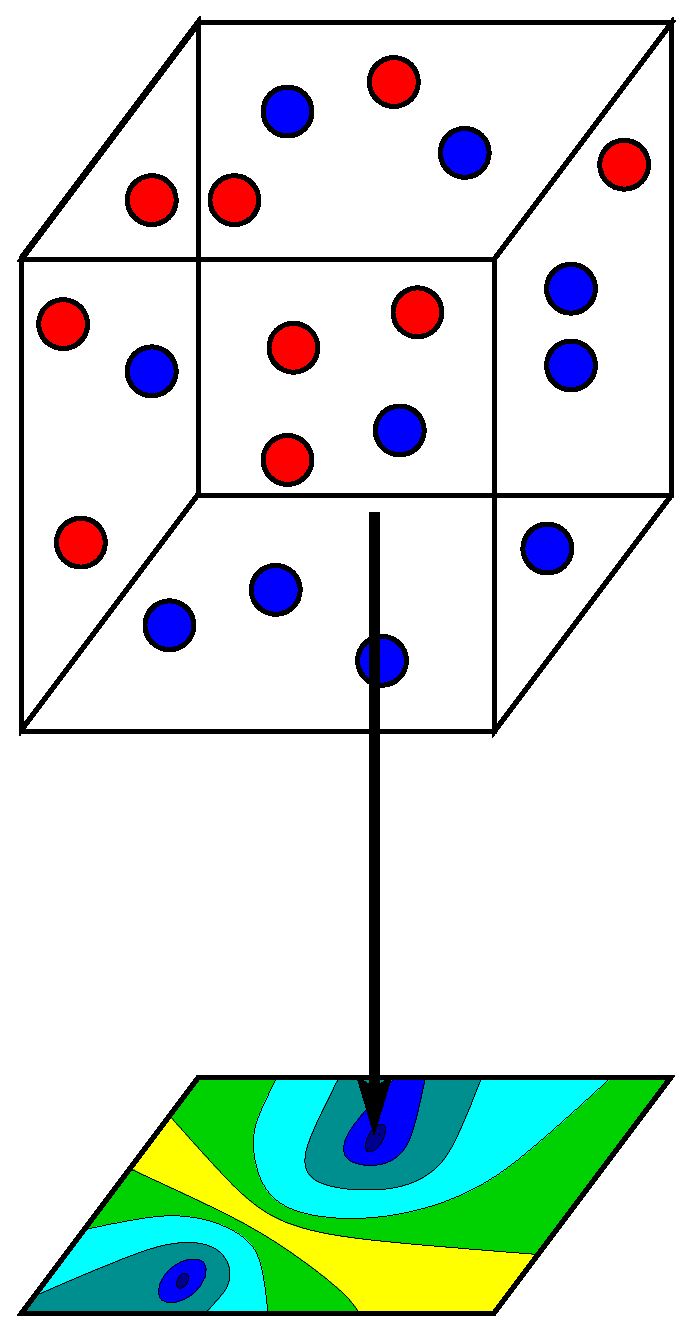
\includegraphics[width=0.35\textwidth]{hmmd-graphic.eps}};
\path(graphic1) ++(2,3) node(label1)[anchor=north west, text width=0.7\textwidth]{Configuration space $\xb \equiv (x_1,y_1,z_1,\dots)$};
\path(graphic1) ++(2,2) node(label1)[anchor=north west, text width=0.7\textwidth]{MD $m_i\ddot{x}_i = -\nabla_iV(\xb) + \mbox{ensemble forces}$};
\path(graphic1) ++(2,1.5) node(label1)[anchor=north west, text width=0.7\textwidth]{Samples $\Rightarrow\ \xb(t_1),\ \xb(t_2),\ \dots$};
\path(graphic1) ++(2,1) node(label1)[anchor=north west, text width=0.7\textwidth]{Ergodicity $\displaystyle\langle X\rangle \approx \frac{1}{n_\tau}\sum_{i=1}^{n_\tau} X[\xb(t_i)]$};
\path(graphic1) ++(0.25,-1) node(label2)[anchor=north west, text width=0.7\textwidth]{Mapping function $\thetab(\xb)\mapsto \zb$};
\path(graphic1) ++(2,-2) node(label3)[anchor=north west, text width=0.7\textwidth]{Feature space $\zb^M \equiv (z_1,z_2,\dots)$};
\path(graphic1) ++(1.5,-3) node(label4)[anchor=north west, text width=0.7\textwidth]{Free energy $F(\zb)=-k_{\rm B}T\ln\langle\delta\left[\theta(\xb)-\zb\right]\rangle$};
\end{tikzpicture}
\end{frame}
